\chapter{MARCO METODOLÓGICO}

\section{Tipo, nivel y diseño de la investigación}
\subsection*{Estudio madre}
El estudio madre de donde provienen los datos es de carácter observacional y consiste en una cohorte prospectiva iniciada en el 2017 en comunidades ganaderas del departamento de Junin bajo el nombre de VIRSEL. Posterior a ello, bajo el nombre de HYCOM, se hizo una segunda recolección de datos en el 2018. Finalmente, este estudio fue modificado en el 2019 ampliando su alcance al eliminar la limitante del departamento; lo cual permitió la recolección de información en la región de Huancavelica en el 2020.

\subsection*{Estudio de tesis}
El estudio de tesis se trata de una investigación de carácter observacional y de corte transversal con la información recolectada en el estudio madre en los centros poblados de Corpacancha y Canchayllo.

\section{Población, muestra y tamaño de muestra}
La población del presente estudio comprende a los habitantes del centro poblado de Corpacancha, Junín-Perú. La información recolectada (muestra) respecto a la tenencia de la enfermedad proviene de dos intervenciones realizadas con anterioridad en la comunidad:
\begin{enumerate}
	\item VIRSEL: Primera intervención realizado en Octubre del 2017. La información fue recolectada por medio de una campaña de despistaje gratuita en el centro de salud del lugar.
	\item HYCOM: Segunda intervención realizada en Junio del 2018. La información fue recolectada por medio de una campaña de despistaje gratuita en la que se visitaron las casas de los habitantes.
\end{enumerate}

Por otro lado, la información referente al otro centro poblado sobre el que se implementará la metodología (Canchayllo, Junín-Perú) proviene de tres intervenciones realizadas en los años 2019 (Septiembre) y 2020 (Diciembre). Esta recolección de información se llevó a cabo gracias al fondo EULAC, a través de CONCYTEC (PRO CIENCIA), quienes también apoyaron esta investigación.

El poder trabajar con información en relación a la tenencia de hidatidosis humana proveniente de dos intervenciones diferentes realizadas con varios meses de diferencias es posible dado al periodo de incubación de la enfermedad (Ver Sección \ref{hidat}). Por otro lado, en lo que respecta a la información sobre la distribución espacial de los habitantes, esta proviene de un censo realizado en la comunidad en simultáneo a los estudios VIRSEL y HYCOM. De este se tienen las coordenadas geográficas de cada casa de la comunidad.
\newpage
\section{Técnicas de análisis e instrumentos}
\subsection{Análisis de datos}
Se inició con una limpieza de la base de datos a fin de contar solo con la información con la que se trabajó, creando las variables necesarias para su procesamiento. Después, se consolidó en una sola base de datos con las coordenadas de cada casa y sus distancias al centro de salud. %El diccionario de las variables de esta base de datos consolidada se encuentra en el Anexo \ref{DicVar}.
Posterior a esto, se procedió a realizar un análisis exploratorio de las variables y los resultados fueron reportados por medio de tablas.\\
Previo al procesamiento de la información real por medio del método planteado, fue necesario estudiarlo. Por ello, su eficacia se evaluó dentro de los siguientes escenarios:
\begin{enumerate}
    \item Densidad poblacional homogénea, riesgo espacial constante
    \item Densidad poblacional heterogénea, riesgo espacial variable
\end{enumerate}
Para cada uno de estos 2 escenarios, las simulaciones se realizaron tomando en consideración diferentes niveles de prevalencia de hidatidosis humana. De igual forma, en cada uno se simularon dos tipos de muestreos: uno totalemten aleatorio y el otro con un sesgo de selección hacia los más próximos al punto en que se recolectó la información por medio de la campaña. Esto fue considerando diferentes niveles de cobertura (porcentaje de individuos de la población que participaron en la campaña de despitaje). Estos escenarios han sido simulados como procesos puntuales. Estos han sido procesos de Poisson homogéneos y no-homogeneos, según sea el caso constante o variable. Con cada uno de los escenarios simulados, se procedió a estimar la prevalencia por medio del método planteado (ver Sección \ref{enfteocon}). Se comparó el valor de esta estimación con el resultado obtenido por el método tradicional (ver Ecuación \ref{estprop}) y el nivel de prevalencia establecido en cada simulación. Con esto se determinó bajo qué condiciones el método propuesto resulta eficiente en comparación al método tradicional tomando como criterio al ECM de las estimaciones (ver Ecuación \ref{ECM}).\\
Al pasar a la data real, además de utilizar la información obtenida en la intervención VIRSEL por medio de la campaña de salud realizada en el Centro Poblado de Corpacancha (Junín, Perú), se usó la información proveniente del censo realizado a la comunidad para la distribución espacial de los pobladores. A continuación, para determinar la probabilidad de que cada individuo de la comunidad haya participado en la intervención VIRSEL se ajustó un GAM (ver Ecuación \ref{GAM}) con las coordenadas del habitante, considerando también como covariables al sexo y al rango de edad. Después, a fin de tener un control en las estimaciones por ambos métodos, cada una de estas fue comparada con el valor de la prevalencia observada en la intervención HYCOM. Finalmente se implementó el método sobre la población de un centro poblado diferente (Canchayllo) y se obtuvo una prevalencia corregida.\\
El código de lo trabajado en esta sección en R, tanto el análisis como las simulaciones, se encuentra en el QR presentado en el Anexo \ref{CodR}.
\subsection{Instrumentos de medición}
\subsubsection*{Prueba diagnóstica}
Para determinar la tenencia de Hidatidosis Humana en el estudio VIRSEL se empleó la prueba diagnóstica de Wester Blot. Esta prueba consiste en vertir sangre sobre un papel especial y según el número de bandas que esta presenta, se determina si el individuo presenta o no Hidatidosis. Por otro lado, en el estudio HYCOM, la prevalencia de la enfermedad se determinó por medio de una ecografía y una tomógrafia, además del Wester Blot. 
\newpage
\subsubsection*{Geolocalización}
Durante el censo realizado en paralelo se determinó la casa correspondiente para cada individuo de la comunidad. De igual forma, por medio de un equipo de GPS se determinaron las coordenadas para cada casa de la comunidad. Esta información fue almacenada digitalmente en formato KML.
\begin{figure}[h]
\centering
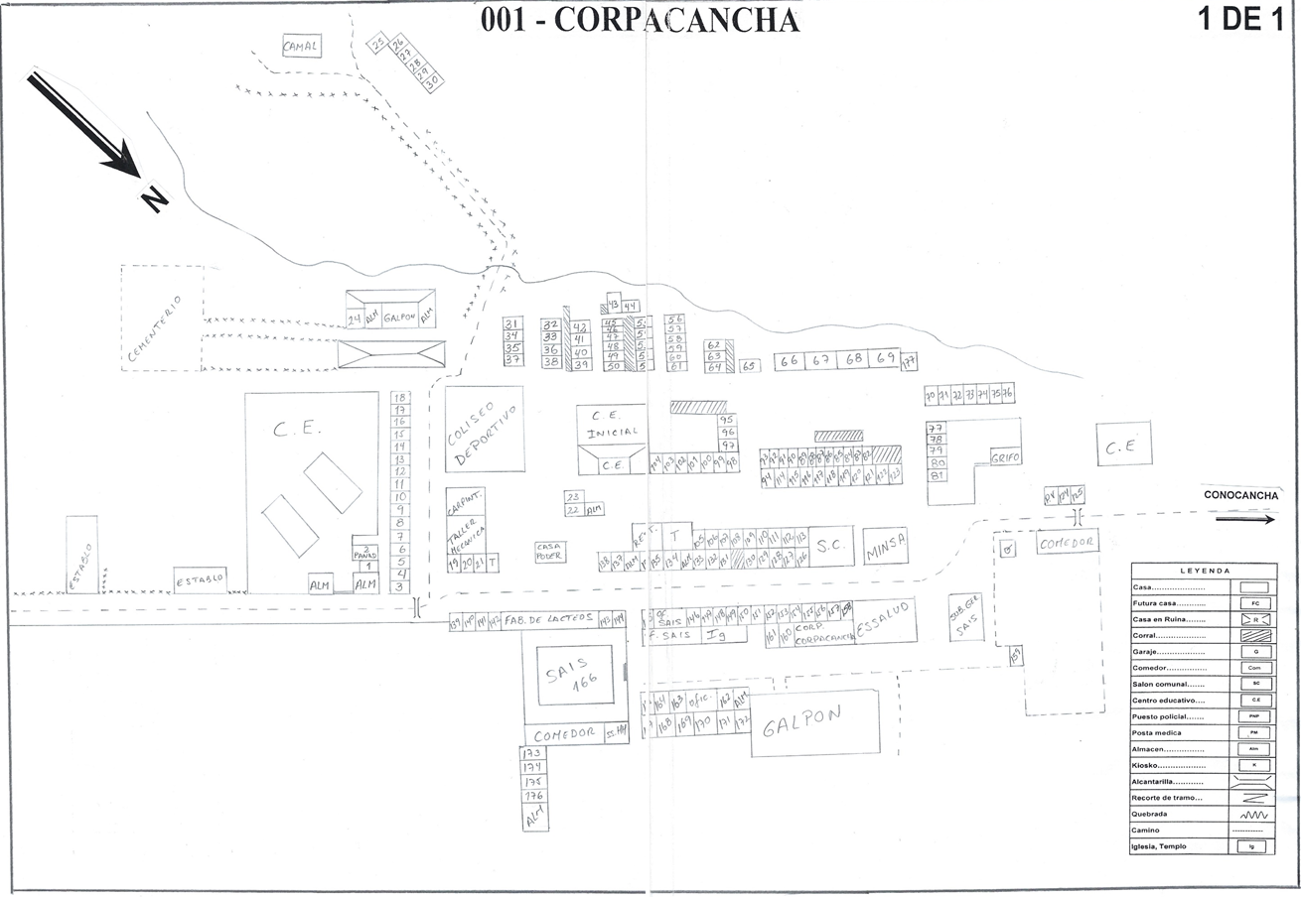
\includegraphics[width=0.5\textwidth]{imagenes/corpacancha_mapa.png} %,angle=180
\caption{Mapa urbano del centro poblado de Corpacancha (Junín, Perú)}
\end{figure}

\newpage

\section{Cuadro de operacionalización de variables}
\begin{table}[htbp]
  \centering
  \caption{Cuadro de operalización de variables}
  \vspace{0.5cm}
    \begin{tabular}{|p{6.355em}|p{11.93em}|p{5.145em}|p{11.215em}|}
    \toprule
    Variable & Definición Conceptual & Tipo  & Valores \\
    \midrule
    Distancia & Distancia en metros desde la casa de un individuo al centro de EsSalud & Continua & Número real mayor a 0 \\
    \midrule
    Prevalencia & Proporción de individuos que presentan la enfermedad & Continua & Número real comprendido entre 0 y 1 \\
    \midrule
    Sexo  & Sexo del individuo & Nominal & 0: Femenino\newline{}1: Másculino \\
    \midrule
    Edad  & Tiempo de vida en años del individuo & Discreta & Número entero mayor o igual a 0 \\
    \midrule
    Rango de edad & Tiempo de vida en años del individuo agrupado en rangos & Ordinal & 1: Menores de 15 años\newline{}2: De 16 a 30 años\newline{}3: De 31 a 40 años\newline{}4: De 41 a 50 años\newline{}5: De 51 a 65 años\newline{}6: De 66 años a más \\
    \bottomrule
    \end{tabular}%
  \label{tab:addlabel}%
\end{table}%



\section{Matriz de consistencia}
En la siguiente página, en la Tabla \ref{matcons}, encontramos la matriz de consistencia del estudio
\newpage
\begin{landscape}

\begin{table}[htbp]
  \centering
  \caption{Matriz de consistencia}\label{matcons}
  \vspace{0.5cm}
    \begin{tabular}{|p{11.07em}|p{11.07em}|r|r|p{11.07em}|}
    \toprule
    \textbf{Problema} & \textbf{Objetivos} & \multicolumn{1}{p{11.07em}|}{\textbf{Hipótesis}} & \multicolumn{1}{p{11.07em}|}{\textbf{Variables e Indicadores}} & \textbf{Metodología} \\
    \midrule
    \textbf{Problema General} & \textbf{Objetivo General} & \multicolumn{1}{p{11.07em}|}{\textbf{Hipótesis General}} & \multicolumn{1}{p{11.07em}|}{\textbf{Variable dependiente}} & \textbf{Tipo de Investigación} \\
    ¿Se puede emplear un método de estimación de prevalencia considerando la distribución espacial para reducir el sesgo del muestreo? & Estudiar un método de estimación de prevalencia considerando la distribución espacial para reducir el sesgo del muestreo & \multicolumn{1}{p{11.07em}|}{El método planteado estima la prevalencia de forma insesgada} & \multicolumn{1}{p{11.07em}|}{Prevalencia: Porcentaje de individuos que presentan la enfermedad} & Básica. \\
    \textbf{Problemas Específicos} & \textbf{Objetivos Específicos} & \multicolumn{1}{p{11.07em}|}{\textbf{Hipótesis Específica}} & \multicolumn{1}{p{11.07em}|}{\textbf{Variable independiente}} & \textbf{Tipo de Investigación} \\
    ¿Cómo se diferencian los resultados obtenidos de las estimaciones de la prevalencia mediante el método clásico y el error de estimación del método propuesto? & Comparar los resultados obtenidos de las estimaciones de la prevalencia por el método tradicional y el método propuesto & \multicolumn{1}{p{11.07em}|}{El método planteado presenta un menor Error Cuadrático Medio en la estimación de la prevalencia que el método tradicional.} & \multicolumn{1}{p{11.07em}|}{Ubicación de la vivienda del individuo} & Observacional. \\
    ¿Cuál es el método adecuado de acuerdo a las condiciones de la investigación? & Determinar el método adecuado de acuerdo a las condiciones de la investigación. & \multicolumn{1}{p{11.07em}|}{El método planteado es el adecuado para la situación que se está observando} & \multicolumn{1}{p{11.07em}|}{Presencia de la enfermedad en el individuo} & A fin de comparar los métodos antes de aplicarlos en la data real, se simularán escenario tomando en consideración diferentes condiciones. \\
    ¿De cuánta es la prevalencia de la hidatidosis humana en el centro poblado de Corpacancha mediante el método propuesto y de cuanta sería en un centro poblado diferente? & Estimar la prevalencia de la hidatidosis humana en el centro poblado de Corpacancha y en un centro poblado diferente mediante el método propuesto. &       &   Covariables epidemiológicas    & La información del caso a tratar proviene de dos campañas médicas realizadas en la comunidad. \\
    \bottomrule
    \end{tabular}
  
\end{table}%

\end{landscape}
